\chapter{Methodologies}
\graphicspath{{Chapter3/Figs/}{Chapter3/Figs/}}

This chapter describes the project-related academic methodologies in the given context of the author and the planned approach to achieve the thesis's goals and objectives. The reader is introduced to the rationale for the intended workflows, hardware, and software tools.

\section{Derivation of the case study}
\label{chapter3-derivation-of-the-case-study}

In October 2021, the author began working as a cloud software engineer at IDUN Technologies to further develop existing software products. IDUN Technologies had already created a PoC software system that included a web-based single-page application (SPA) hosted on AWS Amplify, a backend-as-a-service aiming to simplify the deployment of backends for mobile or web apps. IDUN's in-ear headphone sensor sent EEG data to a network bridge via Bluetooth and then to the cloud via the internet. The raw EEG data was saved and available for download in various file formats.

\begin{figure}[!ht]
  \centering
  
\includegraphics[width=\linewidth]{raw-filtered-data.png}
  \caption{Difference between raw and filtered EEG data from IDUN's in-ear device.}
  \label{fig:raw-filtered-eeg}
\end{figure}

In addition to raw data, the IDUN app provided transformed data, such as, e.g. filtered data, which included low-pass and high-pass filtering of EEG data as shown on \autoref{fig:raw-filtered-eeg}. This transformed EEG data was then saved alongside the raw version on the cloud. The EEG data could also be visualised in near-real-time on the web app as a time-series x- and y-axis plot. Additionally, users could control the device by sending start and stop commands to the hardware components. The architecture overview is displayed on \autoref{fig:idun-amplify} in which IDUN GDK refers to the IDUN Guardian Development Kit.

\begin{figure}[!ht]
  \centering
  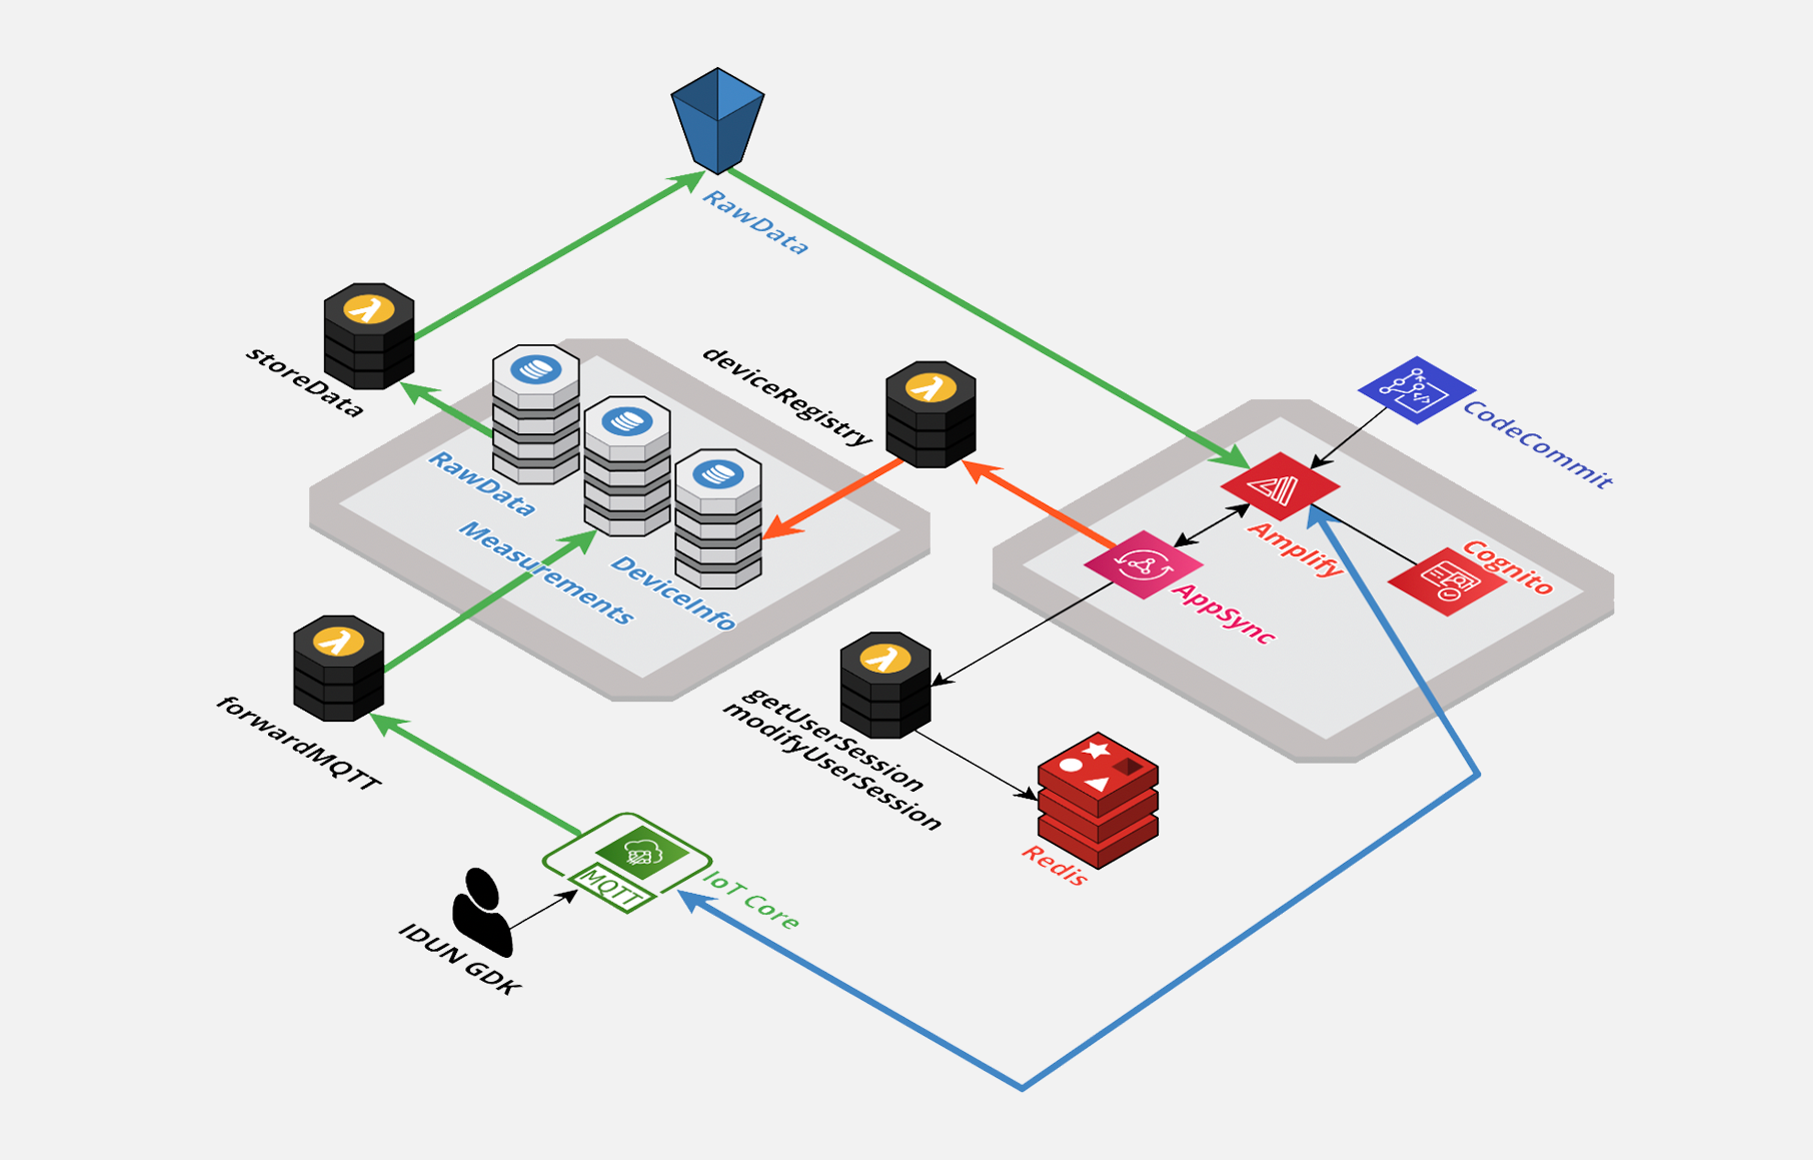
\includegraphics[width=0.75\linewidth]{idun-amplify.png}
  \caption{IDUN's software architecture at the end of 2021.}
  \label{fig:idun-amplify}
\end{figure}

The system was in a relatively unstable state and had strange error sources that made it impossible to reliably record EEG data for more than a few minutes, making the product unusable for existing customers or a mass-market launch. While working on the system, the author encountered various amount of technological flaws and problems as listed in the following list:

\begin{itemize}

\item AWS Amplify is great for frontend developers who want to build simple backends with CRUD\footnote{CRUD is an acronym describing general operations of a backend system: Create, Read, Update and Delete.} operations, but not so good for anything custom, like the streaming-focused aspect of EEG. Therefore, the AWS Amplify system must be abandoned as soon as possible, or a project will be built with the wrong tools and foundations.
\item The network bridge was a Raspberry Pi 4 Model B running uncompiled Python code, which after some analysis, turned out to be the primary source of most of the bugs. The question was raised whether the network bridge was needed since IDUN would become a completely mobile system, either way, not tied to a network and directly connected to a mobile phone or a computer.
\item The cloud's heartbeat functionality was missing, which meant that the cloud knew nothing about the hardware devices, and simply assumed that data would flow in as soon as the start command was sent to the device, creating a pure happy path scenario.
\item The cloud infrastructure was automatically provisioned by AWS Amplify, which uses AWS CloudFormation as its core, which is an infrastructure as code (IaC) tool, that was run inside of AWS CodePipeline, AWS' continuous integration service, which made everything coupled to specific AWS services where the technical decision to use them was not made based on reasoning but based on the Amplify's engineers to use it.
\item All software in the cloud was built using the AWS Console (the AWS graphical user interface). Therefore, no current state in the form of IaC reflected the current infrastructure, which made it impossible to reproduce the cloud in different environments, e.g. prevent blast radius' if something went wrong.
\item The data was streamed via [IBM] MQ Telemetry Transport (MQTT), a publish-and-subscribe transport protocol commonly used for IoT devices that send, e.g. telemetry data regularly. The purpose of MQTT was not to send high-frequency EEG data in real-time but to minimise network bandwidth. Therefore, there was also a need to rethink this technological decision based on the nature of IDUN's EEG sensor, which produces 250 EEG samples per second.
\item The web application was a thick client, meaning that it ran a lot of business logic, such as filtering raw data for real-time visualisation, which was another technological misstep, as the client-side JavaScript ecosystem is far inferior compared to, e.g. the Python ecosystem that could run in the backend to handle such tasks. If possible, shipping business logic that could hold intellectual property to clients should be avoided if possible, especially with a commercial product.
\item The web app was not connected to a single endpoint on the backend and used the MQTT stream and the non-real-time aspects of the app (e.g. login or list of recorded EEG data) via different sources. For example, the MQTT stream was subscribed directly from the device itself and did not run through AWS Amplify's GraphQL API, which made coupling the systems into a coherent and robust API cumbersome.
\item The state of the whole application was difficult to handle due to the decoupled logic from the streaming aspect and standard CRUD operations. Combined with the lack of a hardware heartbeat, it was very tedious to figure out what the user was doing and what was being sent. As an interim solution, AWS ElastiCache, a provisioned service for in-memory databases like Redis, was set up, but the state was traded in the web app and on ElastiCache at the same time. For example, if a user left the web app during a data stream, the stream was stopped, and the EEG data was sent to the void.
\end{itemize}

Due to growing problems with the existing software system and an ever-increasing technical debt as a result of the software not being test-driven or developed without code quality standards, resulting in bugs and quirks that are difficult to track down, the author proposed to halt the implementation of new features and restructure the system from the ground up using a more software engineering-oriented approach. The company's management approved the request for such redevelopment in early December of 2021. At the time the author was already working on his original Bachelor project, which focused on a mind-controlled multiplayer game, assuming that IDUN's software system would be stable by the time the Bachelor project began. The original bachelor project's focus was officially changed at the end of 2021 to create a thesis on this refactored software system.

\section{Case study}
\label{chapter3-case-study}

As mentioned in previous chapters, IDUN manufactures an EEG sensor in the form of in-ear headphones. Their vision is to develop and sell their hardware and license a software product coupled with the hardware. They call it the Neuro-Intelligence Platform (NIP), as shown on \autoref{fig:idun-nip}.

\begin{figure}[!ht]
  \centering
  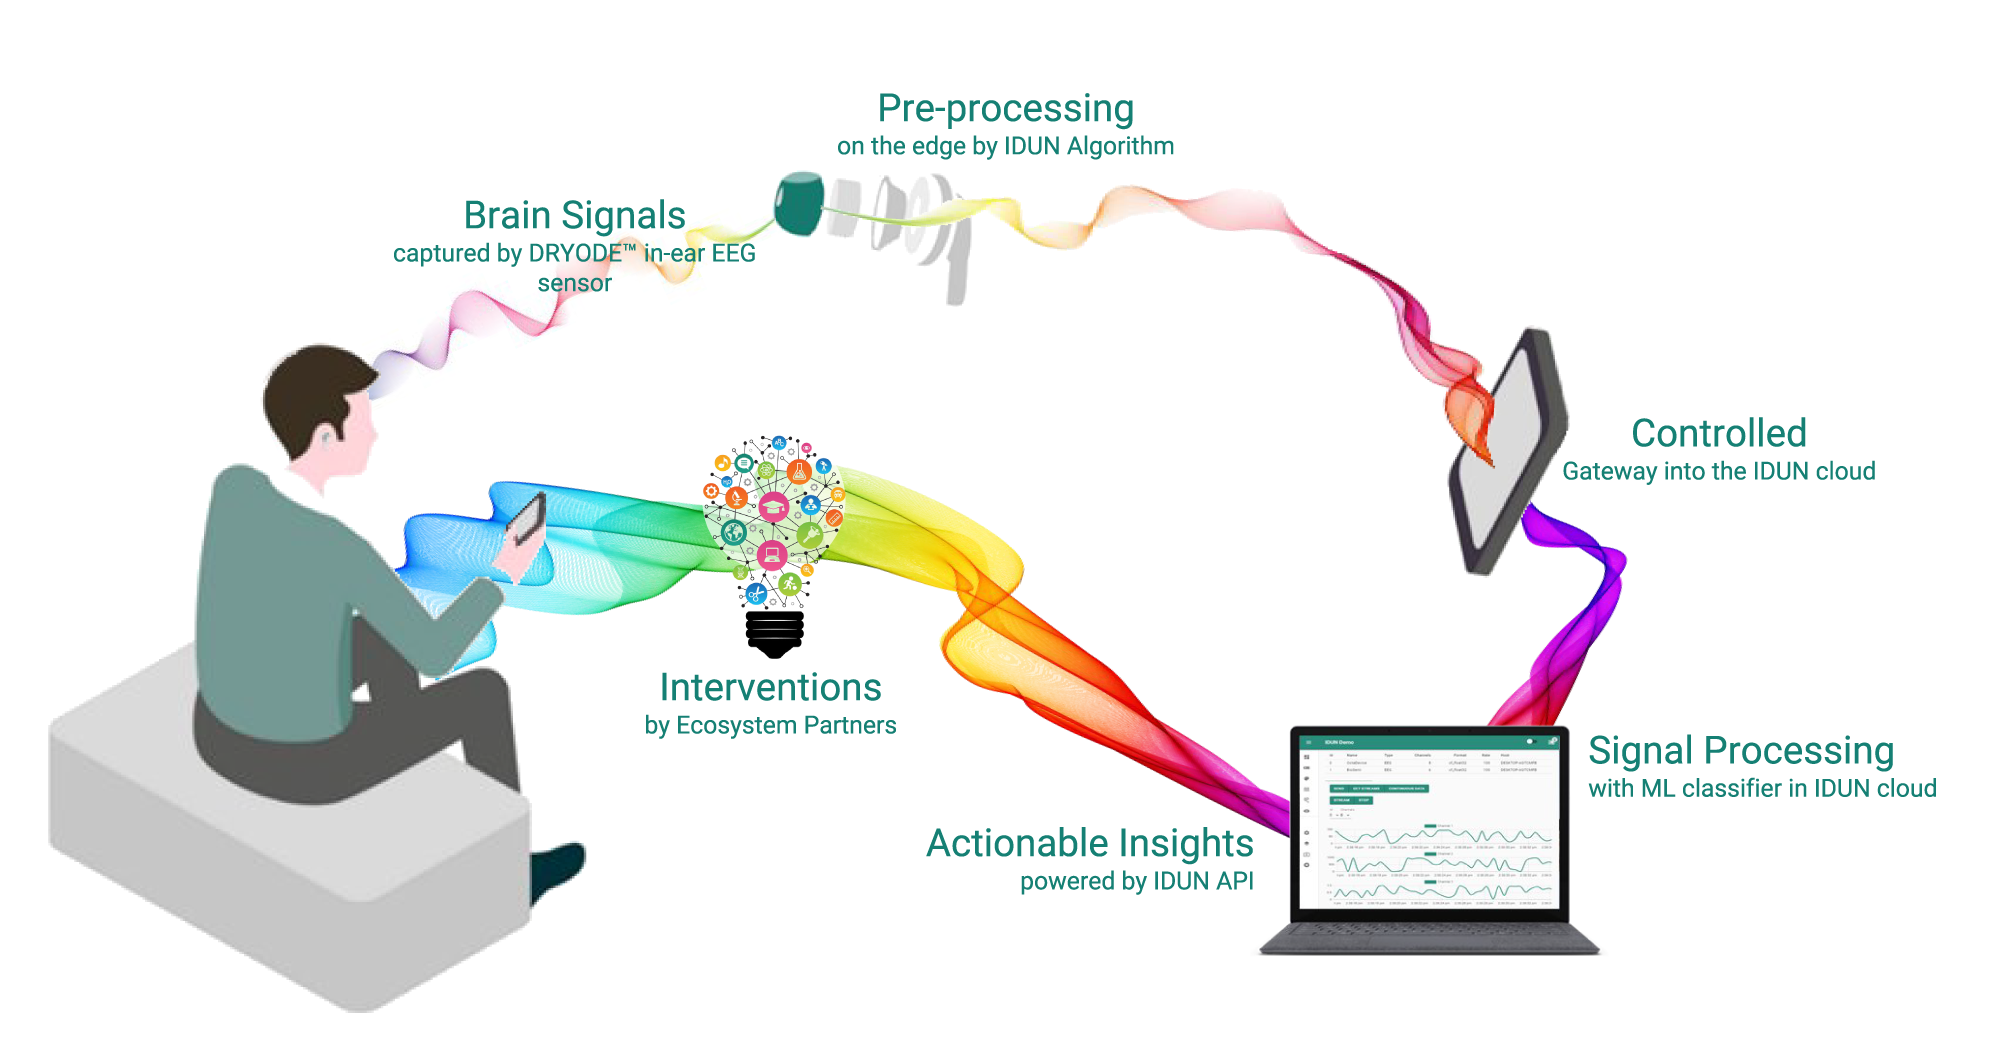
\includegraphics[width=0.8\linewidth]{idun-nip.png}
  \caption{IDUN's depiction of their vision of a closed neurofeedback loop system including the hardware and software.}
  \label{fig:idun-nip}
\end{figure}

The mission is essentially that an unobtrusive BCI device, such as an in-ear headset, can be worn for the majority of the day while measuring neural data that is sent in real time to the cloud to process and classify actionable insights that other developers can use to build their interventions (e.g., apps, websites, and games) on top of it to promote mental health and well-being, as described by IDUN in its vision. Furthermore, the aspect of longitudinal data is important, implying that it could be advantageous to store neural data over a long period of time and run classifiers on it from time to time to better understand one's brain.

It was critical to select an appropriate research method in order to develop a system that would fulfil the company's mission and vision. The author chose a case study because it is an effective method for dealing with unusual and atypical cases while also providing new and unexpected perspectives in certain situations developing something in a company in a real-life scenario.

\section{Procedure}
\label{chapter3-procedure}

This section describes the planned procedure for conducting a case study-based research methodology to develop the proposed software system at IDUN Technologies.

\subsection{Project stages}
\label{chapter3-project-stages}

The goal was to conduct empirical research and examine the use case from various perspectives. In addition, two other methodologies were used in the case study research: 1. User research with experts, ergo expert interviews, which entails locating experts on topics such as EEG on the cloud or BCI software and asking them questions that will assist in answering the research question of this thesis and 2. internal company group discussions. A group discussion aims to learn about other people's attitudes and opinions. As a result, group discussions are ideal for investigating topics such as behaviourally usage concepts and product perception, which align well with IDUN's goals.

% - The study used a between-subject design (treatment group, control group) with the
% depression score on the XXX depression scale as dependent variable.
% - The study used a within-subject design (pre-treatment measurement, post-treatment
% measurement) with the depression score on the XXX depression scale as dependent variable.
% - The study used a mixed design with the between-subject factor group (treatment, control) and the within-subject factor time (pre-treatment, post-treatment). The depression score on the XXX depression scale served as the dependent variable.

% - Three types of materials were used. First,… Second,… Third,…

% - Before the experiment started, participants were randomly assigned to two groups: the X group and the Y group.
% - The experiment consistent of two phases. In the first phase,….. . In the second phase,…. .
% - The order of these two phases was counterbalanced
% - First, participants had to… next… subsequently… finally…
% - Simultaneously,…
% - After participants finished X, they… % Example citation

\subsection{Group discussions}
\label{chapter3-group-discussions}

\subsection{Expert interviews}
\label{chapter3-expert-interviews}

\section{Outcomes}
\label{chapter3-outcomes}

\section{Reflection}
\label{chapter3-reflection}

\section{Further development}
\label{chapter3-further-development}

% - First, they were randomly assigned to treatment and placebo group
% - Both groups: 60 minutes intervention
% - Treatment group: first,… next,…
% - Placebo group: first, …next,…
% - Finally, they filled out the depression questionnaire
% o Did you describe everything that is needed to replicate your research?
% o Did you cite the sources of your methods or paradigms?

\nomenclature[rd]{R\&D}{Research and development}
\nomenclature[nip]{NIP}{Neuro-Intelligence Platform}
\nomenclature[spa]{SPA}{Single-page application}
\nomenclature[mqtt]{MQTT}{[IBM] MQ Telemetry Transport}
